\section{Discussion and Analysis}
\label{sec:discussion}

\quad In this section we discuss the implementation details of the HBlast architecture on FPGA. Detailed reconfiguration performance numbers are reported. 

\subsection{Implementation}
\quad Xilinx ISE was used for implementation. The proposed platform was implemented and hardware validated on a Xilinx VC709 evaluation board containing a Virtex-7 XC7VX690T-2FFG1761C FPGA. The static and reconfigurable regions on the FPGA are shown in \textit{Fig.\ref{fig:regions}}. 
\\
\subsection{Resource utilization}
Resource utilization is shown in \textit{Table \ref{tab:util}}. On the Virtex-7 FPGA the platform consumes about \% of logic and BRAM utilization is about \%.

\begin{table}[!t]
\caption {Table Title} \label{tab:util}
\begin{tabular}{l|l|l|l}
\hline
FPGA module        & Slice LUTs & Slice Regs & Block RAM Tile \\ \hline
HBlast             & 11430      & 10738      & 1              \\
bridge             & 68         & 641        & 0              \\
memoryInt          & 5321       & 4809       & 0              \\
Expand             & 2342       & 2410       & 0              \\
hitMem             & 2958       & 808        & 0              \\
queryB             & 39         & 612        & 0              \\
u\_mig\_7series\_0 & 6002       & 4676       & 1              \\ \hline

\end{tabular}
\end{table}



\begin{table}[]
\begin{center}
\caption {Resource Utilization per Module} \label{tab:Util}
\scalebox{1.25}{
\begin{tabular}{|l|l|l|l|}
\hline
Name       & LUTs & FF & BRAM \\ \hline
bridge     & 66   & 642        & 0          \\
memoryInt  & 3165 & 4821       & 0          \\
Expand     & 2980 & 2451       & 0          \\
highScore  & 381  & 697        & 0          \\
hitMem     & 3134 & 1320       & 0          \\
comparator & 10   & 1          & 0          \\
dbShiftReg & 531  & 532        & 0          \\
queryB     & 196  & 612        & 0          \\ \hline
\end{tabular}}
\end{center}
\end{table}

\begin{table}[]
\begin{center}
\caption {Resource Utilization of the Architecture} \label{tab:util2}
\scalebox{1.25}{
\begin{tabular}{|l|l|l|l|}
\hline
Resource & Estimation & Available & Utiliztion \% \\ \hline
LUT      & 5428       & 433200    & 1.25          \\
FF       & 6062       & 866400    & 0.70          \\
IO       & 104        & 850       & 12.24         \\ \hline
\end{tabular}}
\end{center}
\end{table}



\subsection{Timing analysis}

In VC709 board system clock is 200MHz generated by frequency oscillator. Therefore, there is no slack  the maximum frequency will be same as the oscillators frequency. \textit{Table \ref{tab:timingSlack}} shows the timing report of our design. 


\begin{table}[]
\begin{center}
\caption {Time and Frequency Characteristics} \label{tab:timingSlack}
\scalebox{0.85}{%
\begin{tabular}{|l|l|l|l|}
\hline
Total slack, ns & Required time, ns & Arrival time, ns & Maximum frequency, MHz \\ \hline
-0.76           & 5.000             & 5.76           & 173.6                  \\ \hline
\end{tabular}}
\end{center}
\end{table}


The latency is a duration of taken time, which starts right after the reading query and ends when the search is complete. When the device starts reading the register, where query is stored, it waits until the signal that indicates the validity of query comes. Once the \textit{queryValid} flag is high, the process of searching for the hits/matches is initiated, and it lasts until the end of the algorithm. In the architecture, the expansion process takes much more time than the finding the hit. In expansion process, if the exact match is found in the middle of the of 512-bits, that is there are at least 200 bits before or after the location of the match, the former or latter 512-bits of the database in DDR is not retrieved. Otherwise, if that condition is not hold, DDR will be accessed one more time to retrieve the additional 512-bits to allow the range of expansion be sufficient for search operation. Indeed, access time to DDR is relatively long process.


The proposed architecture was examined under two scenarios to identify the dependence of latency on the characteristics of the search in database. The first scenario was to determine the relationship between the latency and the location of the exact match in database. As it is depicted in Fig.\ref{fig:plot1}, x-axis represents the location of exact match in database, and y-axis shows the corresponding time to complete the search. The matches are located in different 512-bits in database, thus, the matches are found in only a certain read operation from the database. The first point in the plot, refer to Fig.\ref{fig:plot1}, indicates the latency when the match is located in the first 512-bits of the database. The rest of the points, similarly, represents that the matches are located in second, third, forth, fifth and sixth 512-bits of the database respectively. It can be clearly seen that the latency for the first case (match in first 512-bits of database) differs from others. The latency in the first case is approximately 6.5 msec, and in the rest of cases it is roughly 8.6 msec. The difference in latency can be explained by the fact that the match is located in the first half of the 512-bits of the database. Thus, there is no information available before these 512-bits, as a consequence DDR is accessed only once and the expansion takes place only in that particular sequence. In the rest of the cases, there is additional information  to retrieve from the DDR, so there are 2 accesses made to DDR. Hence, the latency is longer that the first case.


\begin{figure}
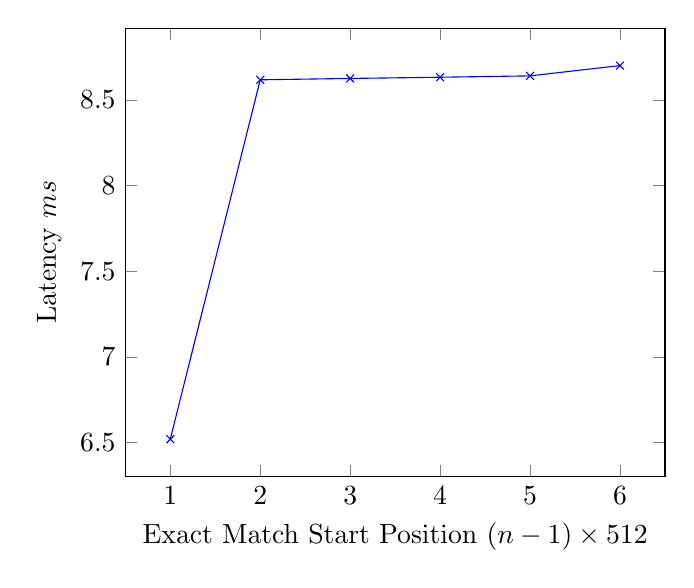
\begin{tikzpicture}
	\begin{axis}[
		xlabel=Exact Match Start Position $(n-1)\times 512$,
		ylabel=Latency $ms$]
	\addplot[color=blue,mark=x] coordinates {
		(1,6.52)
		(2,8.617)
		(3,8.625)
		(4,8.632)
		(5,8.64)
		(6,8.70)
	};
	\end{axis}
\end{tikzpicture}
\caption{Relationship between latency and position of exact match of sequence in database} \label{fig:plot1}
\end{figure}

The second scenario was to test the architecture by increasing the number of matches between query and database. It can be seen in Fig.\ref{fig:plot2} that the latency for the smallest number of matches is the lowest, and as the number of matches increases the latency becomes larger. Due to the fact that each subsequent case of increasing the number of matched W-mers is conducted by adding the short sequence of match, the difference between the latency does not increase dramatically. However, there is a clear tendency of latency to increase with the number of matches. The reason of the difference of the first case form the rest is the same as it was discussed in previous case scenario: the expansion process does not access DDR twice, because there is no available information before the first 512-bits of database. 


\begin{figure}
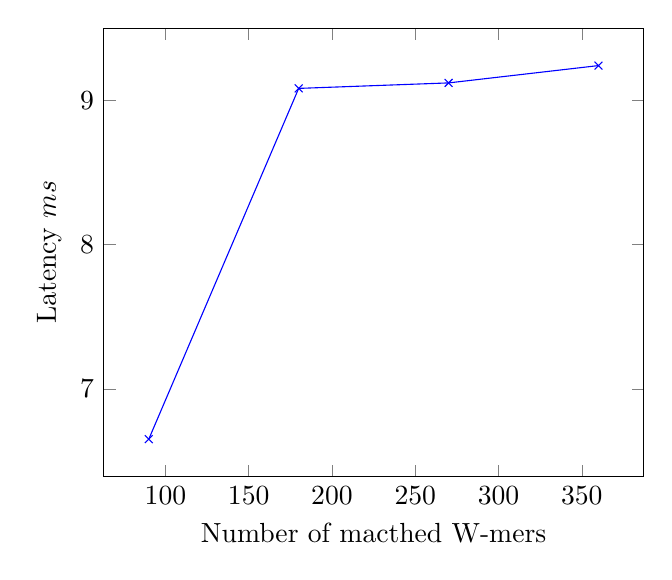
\begin{tikzpicture}
	\begin{axis}[
		xlabel=Number of macthed W-mers,
		ylabel=Latency $ms$]
	\addplot[color=blue,mark=x] coordinates {
		(90,6.652)
		(180,9.082)
		(270,9.12)
		(360,9.24)
	};
	\end{axis}
\end{tikzpicture}
\caption{Relationship between latency and number of exact match of sequence in database} \label{fig:plot2}
\end{figure}